\documentclass[conference]{IEEEtran}
\IEEEoverridecommandlockouts
% The preceding line is only needed to identify funding in the first footnote. If that is unneeded, please comment it out.
\usepackage{cite}
\usepackage{amsmath,amssymb,amsfonts}
\usepackage{algorithmic}
\usepackage{graphicx}
\usepackage{textcomp}
\usepackage{xcolor}
\def\BibTeX{{\rm B\kern-.05em{\sc i\kern-.025em b}\kern-.08em
    T\kern-.1667em\lower.7ex\hbox{E}\kern-.125emX}}
\begin{document}

\title{Conference Paper Title*\\
{\footnotesize \textsuperscript{*}Note: Sub-titles are not captured in Xplore and
should not be used}
\thanks{Identify applicable funding agency here. If none, delete this.}
}

\author{\IEEEauthorblockN{1\textsuperscript{st} Given Name Surname}
\IEEEauthorblockA{\textit{dept. name of organization (of Aff.)} \\
\textit{name of organization (of Aff.)}\\
City, Country \\
email address or ORCID}
\and
\IEEEauthorblockN{2\textsuperscript{nd} Given Name Surname}
\IEEEauthorblockA{\textit{dept. name of organization (of Aff.)} \\
\textit{name of organization (of Aff.)}\\
City, Country \\
email address or ORCID}}

\maketitle

\begin{abstract}
This document is a model and instructions for \LaTeX.
This and the IEEEtran.cls file define the components of your paper [title, text, heads, etc.]. *CRITICAL: Do Not Use Symbols, Special Characters, Footnotes, 
or Math in Paper Title or Abstract.
\end{abstract}

\begin{IEEEkeywords}
component, formatting, style, styling, insert
\end{IEEEkeywords}

\section{Introducción}
....
Según  \cite{Hebert2022}, asdasdads
.

Este artículo se estructura de la siguiente forma. Sección~\ref{sec:MT} presenta las bases de.... Secciób~\ref{sec:Res} destaca los principales resultados de este trabajo. Sección~\ref{sec:TR} describe trabajos relacionados con el foco de investigación de estre trabajo. Finalmente, Sección~\ref{sec:Conclusiones} entrega las ideas finales y trabajos futuras de este trabajo de investigación.

\section{Marco teórico} 
\label{sec:MT}
\subsection{Tema 1}

\subsection{Tema 2}

\subsection{Tema 3}

\section{Resultados}
\label{sec:Res}
\subsection{Resultados 1}

\subsection{Resultados 2}

\begin{itemize}
\item T1.
\item T2.
\item T3.
\end{itemize}

Tabla~\ref{tab:1}
Fig.~\ref{fig:1}

\begin{table}[htbp]
\caption{Table Type Styles}
\begin{center}
\begin{tabular}{|c|c|c|c|}
\hline
\textbf{Table}&\multicolumn{3}{|c|}{\textbf{Table Column Head}} \\
\cline{2-4} 
\textbf{Head} & \textbf{\textit{Table column subhead}}& \textbf{\textit{Subhead}}& \textbf{\textit{Subhead}} \\
\hline
copy& More table copy$^{\mathrm{a}}$& &  \\
\hline
\multicolumn{4}{l}{$^{\mathrm{a}}$Sample of a Table footnote.}
\end{tabular}
\label{tab:1}
\end{center}
\end{table}

\begin{figure}[htbp]
\centerline{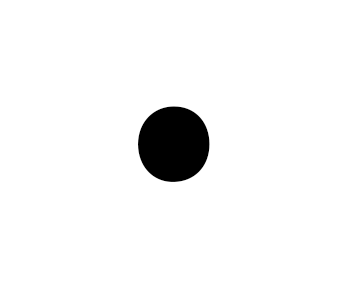
\includegraphics{Figures/fig1.png}}
\caption{Figura Ejemnplo.}
\label{fig:1}
\end{figure}


\section{Trabajos Relacionados}
\label{sec:TR}
...


\section{Conclusiones}
\label{sec:Conclusiones}
...

\bibliographystyle{IEEEtran}  
\bibliography{EjemploBIO}

\end{document}
